\documentclass[12pt, a4paper]{article}

%los use packages van aquí
\usepackage[english]{babel}
\usepackage[utf8]{inputenc}
\usepackage{amsfonts}
\usepackage{amsmath}
\usepackage{amssymb}
\usepackage{tabularx}
\usepackage{listings}
\usepackage{graphicx}
\usepackage[dvipsnames]{xcolor}
\usepackage{setspace}
%\usepackage[left=2.54cm, right=2.54cm, top=2.54cm, bottom=2.54cm]{geometry}
\usepackage[left=3cm, right=3cm, top=3cm, bottom=3cm]{geometry}
\usepackage{xcolor}
\usepackage{float}
\usepackage{hyperref}

\definecolor{backcolour}{rgb}{0.95,0.95,0.92}
\definecolor{codegreen}{rgb}{0,0.6,0}

\lstdefinestyle{mystyle}{
	backgroundcolor=\color{backcolour},   
	commentstyle=\color{gray},
	keywordstyle=\color{codegreen},
	numberstyle=\tiny\color{codegreen},
	stringstyle=\color{magenta},
	basicstyle= \ttfamily,
	breakatwhitespace=false,         
	breaklines=true,                 
	captionpos=b,                    
	keepspaces=true,                                   
	showspaces=false,                
	showstringspaces=false,
	showtabs=false,                  
	tabsize=2,
	numbers=left
}

\lstset{style=mystyle}

\setlength{\parindent}{1em}
\setlength{\parskip}{1em}
\renewcommand{\arraystretch}{1.5}

\title{Exploration of Parkinson's disease recognition space by artificial neural networks.}
\author{Mario Rojo Vicente}
\date{}	 							%fecha de entrega

\addto\captionsenglish{\renewcommand*\contentsname{\LARGE Summary}} %cambia nombre del índice

\begin{document}
	
	 \begin{titlepage}
	\begin{center}
		{\huge \textbf{Technical University of Madrid}}\\
		\vspace{5mm}
		{\large \textbf{Engineering the future}}\\
		\vspace{5mm}
		\begin{figure}[h]
			\centering
			
\includegraphics[height = 8cm]{img/insigneaUPM.jpg}
		\end{figure}
		\vspace{5mm}
		{\LARGE \textbf{Computer Systems Department}}\\
		\vspace{5mm}
		{\large \text{Higher Technical School of Computer Systems Engineering}}\\
		\vspace{5mm}
		\textcolor{RoyalBlue}{\rule{\linewidth}{0.75mm}}\\
		\vspace{2mm}
		\begin{spacing}{1.5} %solo si el título tiene más de una linea
			{\Large \textsc{Exploration of Parkinson's disease recognition space by artificial neural networks.}}
		\end{spacing}
		\textcolor{RoyalBlue}{\rule{\linewidth}{0.75mm}}\\
		\vspace{1cm}
		{\Large \text{Writen by:}}\\
		\vspace{5mm}
		{\Large \textbf{Mario Rojo Vicente}}\\
		\vspace{5mm}
		{\Large \text{Directed by:}}\\
		\vspace{5mm}
		{\Large \textbf{Francisco Díaz Pérez}}\\
		\vspace{5mm}
		{\Large \text{Bachelor Thesis for the Software Engineering Degree}}\\
		\vspace{5mm}
		{\Huge \textbf{June 2022}}
	\end{center}
\end{titlepage}
	
	\section*{}
	\begin{flushleft}
		\vspace*{\fill}
		To Francisco Díaz Perez, that not only helped me by directing this project but was the original creator of the idea behind it and kindly allowed me to further develop it under his close watch, to Rubén Rincón Blanco and Daniel Rebollar Medina who kindly shared their knowledge and experience with me in the complex but beautiful world of Machine Learning, and last but not least to my always loving family without whose unconditional support I could have never achieved the feat of completing this paper. To all of you I express my sincerest gratitude from the bottom of my heart.
		\vspace*{\fill}
		
	\end{flushleft}

	\clearpage
	
	\section*{Abstract}
	
	This paper focuses on the objective a Machine Learning model to classify the advancement of Parkinson´s Disease on a patient given some audio recordings and general information, such as age and gender. For this we will utilize a dataset extracted from synapse to train the several proposed models and finally extract conclusions on the outcomes. This project focuses on the implementation of CNN models based of the VGG-16 architecture. The results ranges from a 30\% accuracy to around a 60\% on all three datasets (train, validation and test) depending on the model and its hyper parameters, as well as the processes applied on the data. In conclusion the project was lacking more instances of reliable data but shows the possibilities of implementing such models on bigger datasets with rather significant results. The final results of this paper allow us to define rules and procedures to be implemented in similar future projects.
	
	%purpose, method, scope, results, and conclusion
	
	\clearpage
	
	\tableofcontents
	\listoffigures
	
	\clearpage
		
	\section{Introduction}
	
	\subsection{Context}
	
	The origin of Parkinson´s disease is at best unclear. While some authors claim it to be a consequence of unknown toxins introduces in the XIX century during the Industrial Revolution, many historical evidences suggest that the presence of this ailment goes as far back as the 2000-1500 ac, when some of its symptoms where first references in the Vedas texts. Further references to what could possibly be Parkinson´s disease were also found in Egyptian papyrus and ancient Chinese medical treaties, among other historical documents. Also, several historical personalities, such as Hipocrates, an ancient Greek´s doctor, and the Italian genius Leonardo Da Vinci, analyzed and studied several symptoms related to this illness.
	
	The first publication referencing what we currently know as Parkinson´s disease was a paper by the name "An essay on the shaking palsy", published in 1817 by the British surgeon James Parkinson. None the less, the disease did not get its final name until the year 1880 when Jean-Marie Charcot, a well recognized french neurologist that was researching the stiffness related to the shaking palsy, proposed to rename the disease in honor of his English colleague.\cite{parkinsonhistoria}
		
	In "An essay on the shaking palsy" James Parkinson referred to the shaking palsy as an "Involuntary tremulous motion, with lessened muscular power, in parts not in action and even when supported; with a propensity to bend the trunk forwards, and to pass from a walking to a running pace: the senses and intellects being uninjured"\cite{parkinson2002essay}. Nowadays the definition for Parkinson´s disease establishes it as a progressive multi-system neurodegenerative disorder more common among people in later years of live, and several studies refer to it as the second most common neurodegenerative illness worldwide.\cite{sveinbjornsdottir2016clinical}
	
	In modern medicine it is a common practice among physicians to refer to the mnemonic TRAP (Tremor, Rigidity, Akinesia and Postural Instability) when diagnosing the Parkinson´s disease, which includes definitions for all it´s main clinical features. Even though nowadays Parkinson´s disease is far more established and recognized, it´s correct and early diagnosis still represents a challenge as many of its signs and symptoms are often insidious. Even when referring to the TRAP, many of its symptoms can only be identified through some sort of examination that will normally not be considered unless specifically looking for those. Some of the symptoms of Parkinson´s disease that are easier to detect are the following:\cite{frank2006approach}
	
	\begin{itemize}
		
		\item The Gait of patients with Parkinson´s disease. Which is characterized for the forward flexion of the trunk and a decrease in the length and height of step. This characteristics can be noticed even before the appearance of the postural instability, but can easily be confused with the symptoms of the senile gait related to the aging process.
		
		\item The development of a masklike face, also known as hypomimia, which is composed of two main factors. A decrease in the blink frequency of the patient and an increased dabbing or drooling due to the difficulty of swallowing saliva that patients of Parkinson´s disease and other parkinsonian illnesses experiment.
		
		\item The development of micrography, which can be identified by a doctor observing a patient do a written task or even by the sufferer himself.
		
		\item The suffering of depression, which is the most common psychiatric feature present in the early stages of the Parkinson´s disease.
		
		\item The development of dementia which is more of a complication common in  the later stages of Parkinson´s disease.
		
	\end{itemize}
		
	When taking about Parkinson´s disease we must realize that it´s early detection has a mayor impact on the ability to control it´s development. Nowadays, newer means of technology allow for newer approaches regarding the diagnosis of Parkinson´s disease, and so many later papers focus on the possibility of relying on Artificial Intelligence and Machine Learning to establish patterns based on the parametrization of different data related but not limited to aspects such as the phonic and kinematic disorders that are attributed to this illness. 
	
	
	
	

	\clearpage
		
	\subsection{Objective}
	
	The main objective is this paper is to implement a convolutional neuronal network based system for the early detection of Parkinson´s Disease based on the parametrization of audio recordings. In order to do so I will based my research on data taken out from Synapse Project. \cite{synapse}
	
	This objective can be therefore subdivided in the following:
	
	\begin{enumerate}

		\item Get familiarized with the Python programming language and the Jupiter Notebook environment.
		
		\item Learn the possibilities offered by python´s deep learning API keras.
		
		\item Research the state of art concerning both the possible structures for Neuronal Networks that could be relevant for this project, as well as previous researches on this topic.
		
		\item Analyze the raw audio data in order to extract the relevant information to then feed into the Neuronal Networks.
		
		\item Implement, train and compare the results of different Neuronal Network´s architectures, in order to provide evidence of their effectiveness regarding the early detection of Parkinson´s Disease based on the provided information.
		
		\item Draw conclusions based on the results of the experiments and provide this information so further research can be realized if the results end up been encouraging.
		
	\end{enumerate}

	To facilitate this projects success I will also establish the following "Machine Learning Project Checklist" as suggested by Aurélien Géron in his book "Hands-On Machine Learning with Scikit-Learn, Keras, and TensorFlow" \cite{handsonmachinelearning}:
	
	 \begin{enumerate}
	 	\item Frame the problem and look at the big picture.
	 	
	 	\item Get the data.
	 	
	 	\item Explore the data to gain insights.
	 	
	 	\item Prepare the data to better expose the underlying data patterns to Machine Learning algorithms.
	 	
	 	\item Explore many different models and shortlist the best ones.
	 	
	 	\item Fine-tune your models and combine them into a great solution.
	 	
	 	\item Present your solution.
	 \end{enumerate}
	
	
	\clearpage
	
	\subsection{Document Structure}
	
	Following this introduction the paper will be structured according to the following sections:
	
	\begin{itemize}
		
		
		\item \textbf{Theoretical Foundations:} where we will establish the basics in order to explain why we took most of the relevant decisions of this paper as well as study other possible developments and establish comparisons between those and the one selected.
		
		\item \textbf{Data Set Overview And Preprocessing:} where we will explain all the processes to which the data has been subjected as well as the reasons behind the implementation of every of this processes.
		
		\item \textbf{Implementing the CNN:} where we will explain the implementation process for the models as well as any problems that could arise during their implementation and what we do to try and solve them.
		
		\item \textbf{Conclusions:} where we will summarize the outcomes of this paper as well as analyze any possible flaws and strong points on the implementation of the project and the models implemented. In this section we will also realize a comparative analysis of the different models proposed for the implementation.
		
		
	\end{itemize}

	\clearpage
	
	\subsection{State Of Art}
	
	When regarding the application of machine learning techniques to the diagnosis of Parkinson´s disease there is a wide range of papers that each present their personal take on the matter.
	
	There are several concerns that need to be addressed when approaching this issue from a technological perspective, the first of which would be to decide on the type of data that is going to be fed into the algorithm.
	
	While some papers focus on the parametrization of the speech, such as a``Diagnosis of Parkinson's disease using deep learning and cell phone voice recordings" \cite{deeplearningygrabaciones} others choose to analysis different sources of data that they feel could present interesting patterns. One possibility would be to realize a kinematic analysis of the patient, using data describing motion of upper and lower extremities, as implemented in ``Artificial intelligence for assisting diagnostics and assessment of Parkinson’s disease—A review" \cite{belic2019artificial}, while several studies in the Synapse Project investigate the possibility of diagnosing Parkinson´s Disease through symptoms related to the loss of recent memory as well as the study of the patients manual abilities.
	
	When choosing the data to be sampled for the experiments it is also relevant to consider the pros and cons of selecting numerous sources of data versus choosing to focus on one specific type. For this paper I have decided to focus on studying voice recordings exclusively, as I find those to have great potential. Nonetheless, I will try to identify any possible relations between the outcomes of the machine learning algorithms application, and other data concerning the state of the patients such as several measurements related to the Unified Parkinson's Disease Rating Scale UPDRS. The idea of utilizing speech analysis to detect and track the deterioration associated to the evolution of the disease comes from sysmtoms such as Dysarthria that affect this functions. \cite{cnntoformantmeasures}
	
	After choosing the data, it needs to be analyzed in order to separate all the relevant information from the useless bits and noise, for that we will focus on analyzing sets of traits for the data that have previously proven good efficacy when utilizing IA and Deep learning. This will be later discussed on the \hyperref[sec:Data]{\textbf{Data Set Overview And Preprocessing}} section of this document.
	
	The last thing to do would then be to choose a Neuronal Network architecture to implement, but this will be furthered discussed in the following \hyperref[sec:TheoreticalBases]{\textbf{Theoretical Foundations}} section.
	
	\clearpage
	
	\section{Theoretical Foundations}
	\label{sec:TheoreticalBases}
	
	In this paper we will be working within the field of Machine Learning, so in order to describe it I will refer to Tom Mitchell, who once described Machine Learning as: 
	
	\textit{"A computer program is said to learn from experience E with respect to some task T and some performance measure P, if its performance on T, as measured by P, improves with experience E."}
	\begin{flushright}
		\textit{- Tom Mitchell, 1997 \cite{handsonmachinelearning}}
	\end{flushright}
	
	Within the context of Machine Learning there exits the branch of Deep Learning, which focuses on training Deep Neuronal Networks, this been stacks of artificial neurons that aim to represent, in a very simplified way, the human´s cerebral cortex. Which is relevant because as I will explain on the following subsection I have decided to implement a Convolutional Neuronal Network (CNN) which happens to be one of the main algorithms that belong to this category of machine learning.
	
	%Applying ML techniques to dig into large amounts of data can help discover patterns that were not immediately apparent. This is called data mining.
	
	\clearpage
	
	\subsection{Types of Machine Learning Systems }
	
	When working with Machine Learning Systems (MLS) there are several questions that have to be answered in order to decide what type of systems best fits the problem at hand: \cite{handsonmachinelearning}
	
	\begin{itemize}
		
		\item Will the system be trained with or without human supervision ?
		
		\item Will the system be able to learn incrementally on the fly ?
		
		\item Will the system be able to detect patterns and build predictive models ?
		
	\end{itemize}
	
	The answer to the first question will allow as to find which of the following four categories of MLSs best suits our model according to the amount and type of supervision they get during their training process: 
	
	\begin{itemize}
	
	\item \textbf{Supervised Learning:} in this type of training the data used for this purpose is accompanied by the desired outcomes of the system for every data instance to be used as input, those outcomes are often referred to as labels. This category includes machine learning algorithms such as Decision Trees and Support Vector Machines.
	
	\item \textbf{Unsupervised Learning:} in this case the train data set provided to the algorithm it´s fully unlabeled. This category includes machine learning algorithms such as clustering and association rule learning.
	
	\item \textbf{Semisupervised Learning:} as its name suggests, semisupoervised learning is a method that is half way between supervised and unsupervised learning and is most useful when working with partially labeled data sets. This category includes machine learning algorithms such as deep belief networks. The algorithms included in this group are often constructed by combining supervised and unsupervised algorithms.
	
	\item \textbf{Reinforcement Learning:} in this case the MLS, often referred to as agent within this context, will analyze its environment, chose and perform actions and then receive a reward or penalty as a consequence of its interaction with the environment. Some examples of machine learning algorithms that fall within this group are DeepMind’s AlphaGo and many robot´s walking algorithms. 
	
	\end{itemize}

	Following the first, the second question will allows us to differentiate between the following two different groups of algorithms:
	
	\begin{itemize}
	
	\item \textbf{Batch Learning:} that encompasses those algorithms that need to be trained before been released to the public, using all the available data and that will not learn once deployed. This type of training often requires a big amount of resources and time to train and it requires to train and deploy a new stance of the product every time we wish for the MLS to take into account any new data.
	
	\item \textbf{Online Learning:} which includes all the algorithms that have the particularity of been able to learn after their deployment. This group is trained by sequentially feeding it with instances of the data that could be organized in small groups, often called mini batches, or individually. Due to its characteristics the algorithms within this group are often implemented in applications that require a rapid and autonomous adaptation to new incoming data or those that aim to run using limited computing resources.
		
	\end{itemize}
	
	
	Finally the last and third question will help us differentiate between:
	
	\begin{itemize}
		
	\item \textbf{Instance-based learning:} this group focuses on learning all data within the training set by heart and then implementing a measures that establishes the similarity of the new instance to the ones used for training and generalizes based on this measure so it can predict its corresponding outcome.
	
	\item \textbf{Model-based learning:} which instead of predicting the outcomes by learning the training examples uses a model chosen by the architect of the MLS. The architect will often choose a model based on an analysis of the data related to the problem ans their own expertise.
		
	\end{itemize}

	For this paper I plan on implementing a MLS that I will train personally with a fully labeled dataset, that will not be required to learn incrementally on the fly but rather will be trained once and then analyzed and that will work based on intances due to the complexity of the data. It is also relevant to consider that in this case we will be analyzing parameterized audio recordings and that is why I considered it could be interesting to try and implement one of the systems that work best for voice recognition, which I found to be RNNs (Recursive Neuronal Networks), CNNs (Convolutional Neuronal Networks) and Transformers.
	
	Taking all the characteristics from both the project and the dataset into account, as well as the fact that I will be working with audio recordings, I decided that the best MLS for this paper would be a Convolutional Neuronal Network (CNN).
	
	\clearpage
	
	\subsection{The CNN Model and VGG Architecture}
	
	In order to understand what a CNN is, we first need to establish a definition for Neuronal Network. 
	
	Therefore we will establish an Artificial Neuronal Network (ANN) also referred to as Neuronal Network (NN) to be a machine learning model based of the networks of biological neurons found in our brains. This model is constituted by one or more layers of any number of artificial neurons, which are at the same time inspired in their biological counterpart. While the original model came from this biological analogy, with time ANN have deviated further and further away from their biological counterpart and so today some researchers argue that this analogy should no longer be considered appropriate.
	
	Now that we have a basic understanding of what a ANN is be can further delve into our solution by addressing what a CNN truly is and what makes them stand out from other ANN based models.
	
	On 1958\cite{cortex58} and 1959\cite{cortex59} David H. Hubel and Torsten Wiesel, realized several experiments on the structure and working mechanics of the visual cortex of cats. This studies set the foundations of the biological model that later on will serve as analogy for the creation of the Neocognitron\cite{neocognitron} in 1980 which was the predecessor of the more modern CNNs.
	
	CNN architectures are often constructed with several building blocks common to other Neuronal Networks such as \textit{Fully Connected Layers}\footnote{A fully connected layer is a type of layer in which all its neurons are all connected to every element of the input of the layer.} and \textit{Sigmoid Activation Functions}\footnote{The sigmoid function is given by $\sigma(x) = 1/(1+exp(-x))$.}\footnote{An activation function is a function implemented by some artificial neurons to produce its output given a weighted sum of inputs. There are many type of activation functions such as sigmoid and relu. }, but also include two more specialized building blocks the Convolutional and Pooling layers:
	
	\begin{itemize}
		
		\item \textbf{Convolutional Layer:} this new type of layer works by connecting its neurons not the totality of the output of the previous layer, but rather to a smaller rectangular fraction of it, referred to as the neuron´s receptive field. In an image for example a particular neuron could be connected to a grid of $Z \cdot Y$ adjacent pixels. 
		
		\begin{figure}[H]
			\centering
			\label{ConvLayer}
			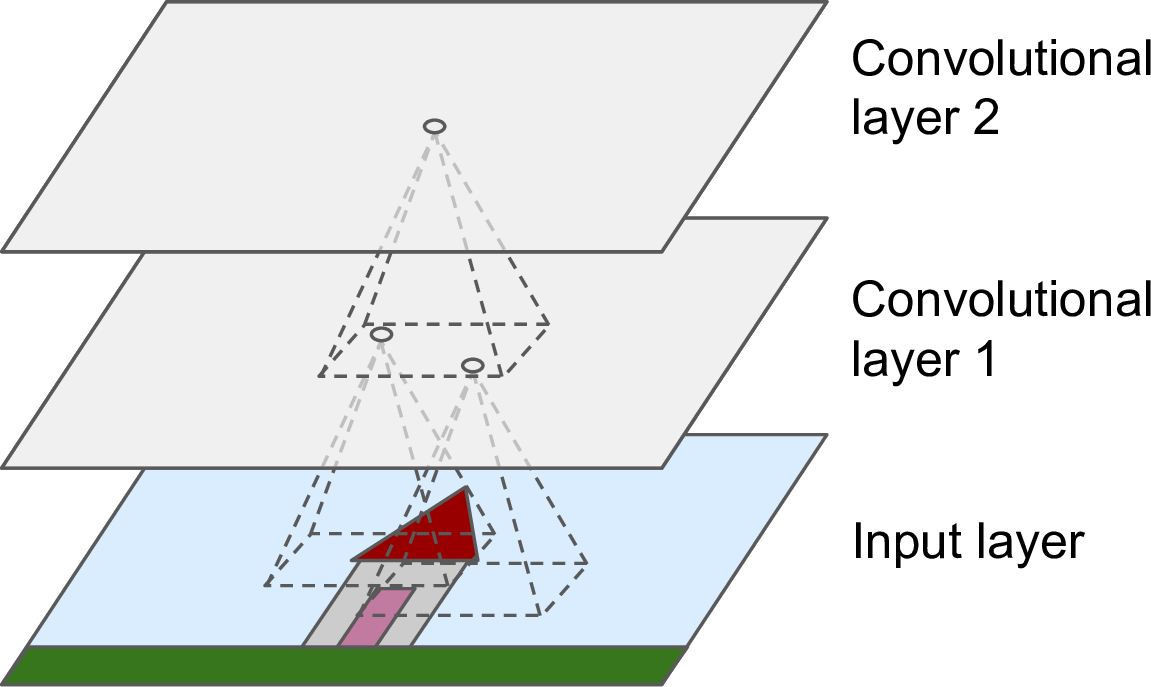
\includegraphics[height=38mm]{img/convLayer.png}
			\caption{Visual representation of the effects of convolution layers.\cite{handsonmachinelearning}}
		\end{figure}
		
		\item \textbf{Pooling Layer:} this layer is often used to reduce the risk of overfitting as well as the computational requirements of any CNN. It works much like the previously described convolutional layer, its objective been to subsample the layer´s input. In this layer the artificial neurons apply an aggregation function such as the max or mean to their input in order to reduce its dimensions,
		
	\end{itemize}
	
	\begin{figure}[H]
		\centering
		\label{MaxPoolLayer}
		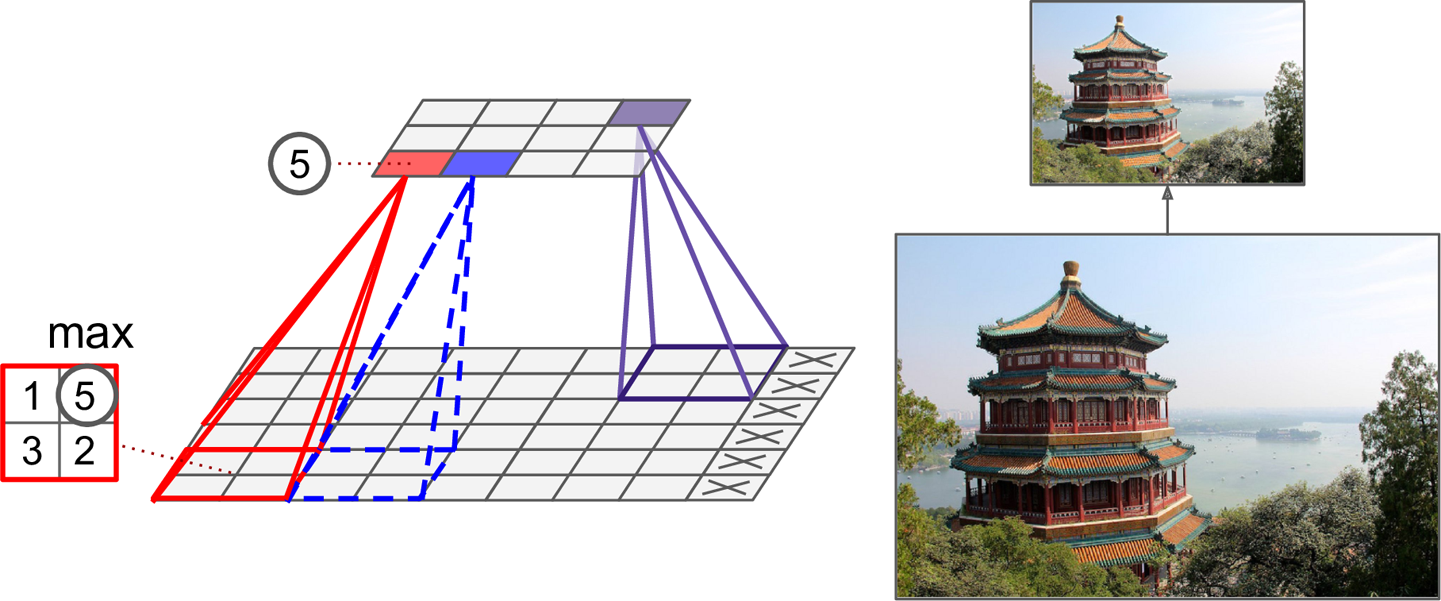
\includegraphics{img/maxPoolingLayer.png}
		\caption{Visual representation of the effects of pooling layers. \cite{handsonmachinelearning}}
	\end{figure}

	After realizing extensive research and discussing with several peers and professors I decided to go with the Visual Geometry Group (VGG) architecture for my neuronal network which focuses on the use of deep convolutional models. Based on this architecture two main models have been established that are referred to by the architecture´s acronym followed by the number of layers they support, those been the VGG-16 and VGG-19 models.\cite{VGGinfo}
	
	\vspace{5mm}
	\begin{figure}[H]
		\label{VGGArchitecture}
		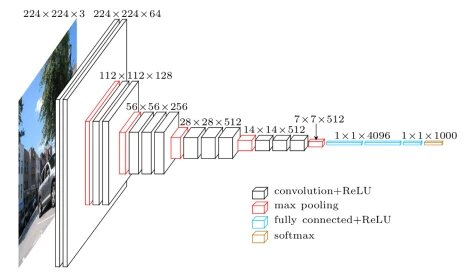
\includegraphics[width=140mm]{img/vgg-neural-network-architecture.jpg}
		\caption{Visual representation of a VGG architecture. \cite{VGGimg}}
	\end{figure}
	\vspace{5mm}

	From the two models previously presented I decided to apply in this paper the VGG-16 architecture, the smaller of the two, as the problem at hand only has a dimensionality of 40 (there are 40 attributes that will be imputed in the network), and if the models turns out to be too big for the problem it could lead to problems such as overfitting.
	
	
	\clearpage
	
	\section{Data Set Overview And Preprocessing}
	\label{sec:Data}
	
	In order to apply any Machine Learning algorithm we need a data set, in this case I will be utilizing one extracted from the Synapse platform. This data set provides 74 different data from a total of 779 participants, all of which has been previously anonymized. From the initial data I will only feed values for the following 40 attributes to the Neuronal Network:
	
	\vspace{5mm}
	
	
\begin{tabularx}{1\textwidth} { 
		| >{\raggedright\arraybackslash}X 
		| >{\raggedright\arraybackslash}X 
		| >{\raggedright\arraybackslash}X 
		| >{\raggedright\arraybackslash}X |}
	\hline
	\textbf{Name} & \textbf{Description} & \textbf{Type} & \textbf{Units} \\
	\hline
	feature01  & Median F0  & real & Hz  \\
	\hline
	feature02  & Mean absolute F0 time derivative  & real & Hz^2 \\
	\hline
	feature03  & Median absolute F0 time derivative  & real & Hz^2  \\
	\hline
	feature04  & Mean absolute value of time derivative of RMS power  & real & Hz  \\
	\hline
	feature5  &Median absolute value of time derivative of RMS power  & real & Hz  \\
	\hline
	feature06-feature19  & Median cepstral coefficients 0-12 for entire voice recording  & real & None  \\
	\hline
	feature20-feature32  & Mean absolute time derivative of cepstral coefficients 0-12 across entire voice recording  & real & None  \\
	\hline
	feature33  & Recurrence period density entropy (RPDE) Hnorm  & real & None  \\
	\hline
	feature34  & Detrended fluctuation analysis (DFA) scaling parameter alpha  & real & None  \\
	\hline
	feature35  & Modified pitch period entropy (PPE)  & real & None  \\
	\hline
	feature36  & Relative spectral power 0-500Hz  & real & None  \\
	\hline
\end{tabularx}

\begin{tabularx}{1\textwidth} { 
		| >{\raggedright\arraybackslash}X 
		| >{\raggedright\arraybackslash}X 
		| >{\raggedright\arraybackslash}X 
		| >{\raggedright\arraybackslash}X |}
	\hline
	feature37  & Relative spectral power 500-1kHz  & real & None  \\
	\hline
	feature38  & Relative spectral power 1kHz-2kHz  & real & None  \\
	\hline
	feature39  & Relative spectral power 2kHz-4kHz  & real & None  \\
	\hline
	current\_age  & Age of participant when call was recorded  & Integer & Years  \\
	\hline
	sex  & Sex of participant  & String & ‘M’/’F’/empty  \\
	\hline
\end{tabularx}


	
	\vspace{5mm}
	
	I have selected all the parameters related to the voice recordings as well as the sex and current age which I believe could be relevant for the classification process.
	 
	Some of the data from the data set that will not be fed to the Neuronal Network relates to the previously mentioned UPDRS (Unified Parkinson's Disease Rating Scale) and will be utilized later on in order to draw any possible relations between those and the outcomes of the Neuronal network. As this data is not directly related to the voice recordings I have not considered it relevant for the inputs of the Neuronal network which affects the gradient.
	
	Previous to its use in the training and validation of the Neuronal Network the data set must be load and go through several processes. In order to load the data I will use python´s Pandas library, which will allow me to generate panda´s data frames from the original coma separated CSV files.
	
	\clearpage
	
	\subsection{Cleaning The Data Set }
	
	The process of cleaning the data will prevent the Neuronal Network from learning any incorrect patterns that may arise of such data and it makes the process of learning more efficient as the incorrect instances would slow down the learning process pushing the weights and bias in wrong directions.
	
	I started the data cleaning process by simply removing all the instances for which the attribute "voice\_code", which can take the values "ok" or "bad", had de "bad" value, as those do not include any values for any of the "features" which are to be imputed in the Neuronal Network. To do so I implemented the following function:
	
	\vspace{5mm}
	
	\begin{lstlisting}[language=Python]
		
	def eliminateBadVoiceCodeElements(data_frame):
			valid_voice_code_elemnts = data_frame.copy()
			valid_voice_code_elemnts = valid_voice_code_elemnts.drop(valid_voice_code_elemnts[valid_voice_code_elemnts["voice_code"] == "bad" ].index)
			return valid_voice_code_elemnts
	\end{lstlisting}
	
	And so before applying the function to the data set we had the following count for the values of the "voice\_code" attribute:
	
	\vspace{5mm}
	
	\begin{lstlisting}[language=Python]
		
	ALL_DATA["voice_code"].value_counts()
	\end{lstlisting}
	
	\begin{figure}[h]
		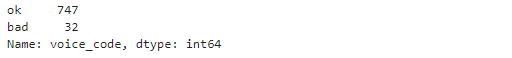
\includegraphics{img/VoiceCodeBefore.png}
	\end{figure}

	And after applying the function to the original data set we ended up with a total of 717 instances after deleting the 32 with value "bad" for the attribute "voice\_code".
	
	In addition of the previous, in order to further clean the data I will proceed by deleting any instances that have an undefined value for any of the attributes. Although in some scenarios those could be considered a valid value for some attributes, given the nature of our features I rather considered them to be failures in the readings. When eliminating the rows with undefined values I did not just limit myself to erasing the ones with an undefined value in one or more of the attributes that would be imputed on the Neuronal Network but rather I eliminated any row with at least one undefined values in any attribute because when considering this to be a failure in the readings I could not trust that the error did not reflect in the values of the other attributes.
	
	This process of deleting the rows with undefined values can be easily done by invoking the dropna method of the pandas dataframe class.
	
	Then, after further analyzing the data I realized that some of the instances had an empty string value for the gender and as I do believe that this could be a significant attribute to input in the neuronal network i decided such value was not valid within this project´s frame and so proceeded with deleting all the instances of data with this value in their sex attribute. In order to do so I implemented he following function:
	
	\vspace{5mm}
	
	\begin{lstlisting}[language=Python]
		
	def eliminateEmptySexElements(data_frame):
		valid_voice_code_elemnts = data_frame.copy()
		valid_voice_code_elemnts = valid_voice_code_elemnts.drop(valid_voice_code_elemnts[valid_voice_code_elemnts["voice_code"] == "" ].index)
		return valid_voice_code_elemnts
	\end{lstlisting}
	
	Finally I also deleted any instances for which the current\_age attribute was lower than the years\_since\_first\_symptom, as such a condition is not logically possible, and also removed all instances with less than 20 as their current\_age value. Which basically eliminated some instances that had a value of 0 for current\_age. I did so with the following function:
	
	\vspace{5mm}
	
	\begin{lstlisting}[language=Python]
		
	def checkAgeIsGraterThanSysptoms(data_frame):
		valid_data_frame = data_frame.copy().reset_index()
		indexes = []
		for index in range(len(valid_data_frame)):
			if valid_data_frame["current_age"][index] < valid_data_frame["years_since_first_symptom"][index] or valid_data_frame["current_age"][index] < 20:
				indexes.append(index)
		valid_data_frame.drop(indexes)
		del valid_data_frame["index"]
		return valid_data_frame
	\end{lstlisting}
	
	\clearpage
	
	\subsection{Normalizing The Data Set And Transforming Non Numerical Values }
	
	Normalizing the data previously to training a Neuronal Network with it bares the benefit of speeding up the learning rates by leading to a faster convergence, this is archived by adjusting the range of values of the different attributes to be the same.\cite{normalization}
	
	In my case I first implemented the min max technique which consists in transforming for every feature it´s minimum value to a zero, it´s maximum value to a one, and then every other value to a decimal between this two.\cite{normalizationTechniques}
	
	\[ x \forall Z \]
	\[ f(x) = (x - MIN(Z))/(MAX(Z)-MIN(Z)) \]
	
	The only significant downside to this technique is the fact that it does not handle outliers well. And according to their plots this would be a problem for several of the features.
	
	We can see the previous problematic represented in the following plot:
	
	\begin{figure}[h]
		\label{Feature02N}
		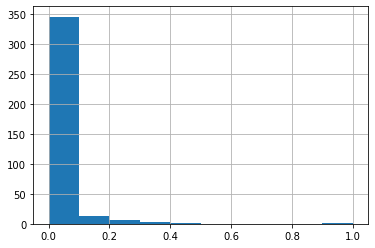
\includegraphics{img/plots/feature02N.png}
		\caption{Histogram for a normalized attribute with outliers. Feature02}
	\end{figure}
	
	In order to minimize the impact of applying the min max technique to those attributes with outliers I decided to apply feature clipping which caps a all features above and below the given boundaries to a fixed value, this on time will help spread the feature values over the entire range. Although this is a helpful technique I did not considered it appropriate for the features which plot shape was similar to the one in Figure 1 and only applied it to some of the attributes with plots that looked similar to the following figure.
	
	\begin{figure}[h]
		\label{Feature24N}
		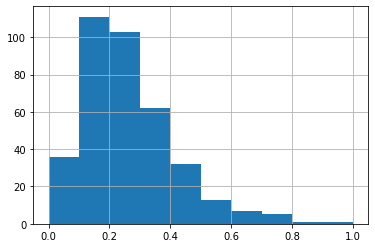
\includegraphics{img/plots/feature24N.png}
		\caption{Histogram for a normalized attribute with outliers. Feature24}
	\end{figure}

	Which after the feature clipping process ended up looking like this:
	
	\begin{figure}[H]
		\label{Feature24NC}
		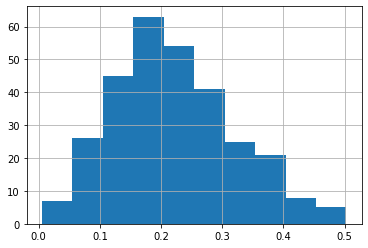
\includegraphics{img/plots/feature24NClip.png}
		\caption{Histogram for a normalized and clipped attribute. Feature24}
	\end{figure}

	In order to archive this improvement in the closeness of the different attributes distributions shapes to a normal distribution I implemented a function based on the Z-Score value of the elements to eliminate any and all outliers of the distribution that showed a relevant degree of skewness whether it is to the right or left.
	
	The formula for the Z-Score is $ Z-Score(x) = (x - \mu)/\sigma $ where $\mu$ stands for the mean and $\sigma$ the standard deviation of the distribution D for which $X \in D$.\cite{datascienceZscore}
	
	\vspace{5mm}
	
	\begin{lstlisting}[language=Python]
		
	def clipZScores(data_frame):
		current_dataframe = data_frame.copy()
		z_scores = zscore(current_dataframe[CLIP_FEATURES])
		abs_z_scores = np.abs(z_scores)
		filtered_entries = (abs_z_scores < 2).all(axis=1)
		new_df = current_dataframe[filtered_entries]
		return new_df
	\end{lstlisting}

	Finally to the several attributes with a value distribution similar to the one presented by ``feature02" I thought about applying Log Scaling, which aims to compress a wide range of values into a smaller range and is nice to use when a handful of the values repeat many times as happens for those attributes.\cite{normalizationTechniques}
	
	\[ \forall x \in Z \]
	\[ f(x) = log(x) \]
	
	It was after my initial attempt that I realized that many of those attributes have features with zero and negative values which actually complicates the application of the Log Scaling and so I decided to try using the RobustScaler and StandardScaler from Python´s sklearn library.
	
	The Robust Scaler uses the same formula $f(x) = (x - M)/(Q3-Q1)) $ where M stands for the median and Q1 and Q3 for the first and third quartiles of a distribution D for which $X \in D$.\cite{normalizeSkLearn}
	
	The Standard Scaler uses the same formula that was implemented for calculating the Z-Score values in the clipZScores function shown above.
	
	\begin{figure}[H]
		\label{Feature03Comparidson}
		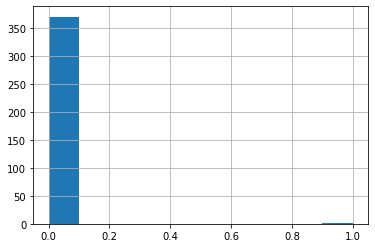
\includegraphics[height=32mm]{img/plots/feature03N.png}
		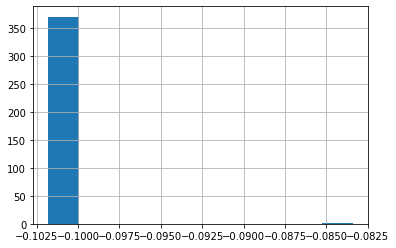
\includegraphics[height=32mm]{img/plots/feature03NStandard.png}
		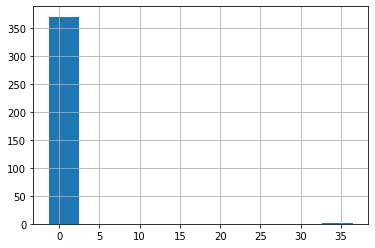
\includegraphics[height=32mm]{img/plots/feature03NRobust.png}
		\caption[width=50mm]{Comparison for normalization applying max min, Robust Scaler and Standard Scaler. Feature03}
	\end{figure}

	As it can be appreciated in the different plots none of the different techniques got a final distribution closer to a normal than the others and so I decided to simply apply max min to all the attributes.
	
	At this point in time I also assigned numerical values to "sex", which happens to be the only non numerical attribute  that was selected as input for the Neuronal Network. This particular attribute only has two possible values after the cleaning process which are "F" for female participants and "M" for male ones, and so the following function assigns the value 1 for male participants and 0 for female ones.
	
	\vspace{5mm}
	
	\begin{lstlisting}[language=Python]
		
	def normalizeSex(data_frame):
		current_dataframe = data_frame.copy().reset_index()
		n_sex = []
		for index in range(len(current_dataframe)):
			if current_dataframe["sex"][index] == "M":
				n_sex.append(0)
			else:
				n_sex.append(1)
		current_dataframe["sex"] = n_sex
		del current_dataframe["index"]
		return current_dataframe
	\end{lstlisting}
	
	\clearpage
	
	\subsection{Splitting The Data Set}
	
	When working with Neuronal Notworks among other machine learning algorithms it is important to prepare several Data sets for the different activities related to the training of the program and the evaluation of its results. In order to do so it is advisable to split the data in the following three different groups:\cite{dateTestsDefs}
	
	\begin{itemize}
		
		\item \textbf{The training data set:} which includes all the data to which the model will be fitted.
		
		\item \textbf{The validation data set:} which includes all the data to be used as reference for the evaluation of a model fit while fine tuning its hyper parameters. The evaluation of the algorithm over this dataset produces the so called data snooping bias which could make it so your predictions are too optimistic.
		
		\item \textbf{The test data set:} which includes all the data to be used as unbiased reference for the evaluation of an already tuned model fit. The evaluation over this dataset can only be affected by the bias derived from choosing some metrics or the others to evaluate the performance of the algorithm.
		
	\end{itemize}

	The creation and implementation of this three groups in the different stages of the training process has the objective of obtaining a final evaluation of the performance of the algorithm as realistic as possible by avoiding any non realistic outcomes that could come from of the over or under fitting of the model to the training data.
	
	Although our dataset came already divided in two files one for train and one for test both files have approximately the same size, 388 elements on the train file and 390 on the one for test, which did not mach the distribution I was looking for. In order to make sets of the sizes I was aiming for I first combined both files into one dataframe and later created the different sets with the following function that I got from the Hands-On Machine Learning with Scikit-Learn, Keras, and TensorFlow \footnote{The function was originally named split\_train\_test but I decided to rename it to something more fitting to its porpouse within the scope of this project.} \cite{handsonmachinelearning}:
	
		\vspace{5mm}
	
	\begin{lstlisting}[language=Python]
		
	def split_dataset(data, test_ratio):
		shuffled_indices = np.random.permutation(len(data))
		test_set_size = int(len(data) * test_ratio)
		test_indices = shuffled_indices[:test_set_size]
		train_indices = shuffled_indices[test_set_size:]
		return data.iloc[train_indices], data.iloc[test_indices]
	\end{lstlisting}
	
	And so after applying all the steps from the previously described data cleaning process I utilized this function to first divide the dataframe containing all the data into the train and validation data sets with a proportion of 80 to 20 and afterwards divide the train data set into the train and test data sets again with the same proportions.
	
	After all of this I ended up with train, validation and test datasets consisting of 238, 74 and 59 elements respectively.
	
	%No incluir en la memoria. More specifically, you train multiple models with various hyperparameters on the reduced training set (i.e., the full training set minus the validation set), and you select the model that performs best on the validation set. After this holdout validation process, you train the best model on the full training set (including the validation set), and this gives you the final model. Lastly, you evaluate this final model on the test set to get an estimate of the generalization error.
	
	\clearpage
	
	\subsection{Generating The Labels}
	
	The final step was then to generate the labels for each feature and for this I decided to create two separate groups. This first one would encompass all elements with a value for the attribute "years\_since\_first\_symptom" grater than 0 and the second one  would be its complementary. Finally I labeled all the elements within the firsts group with a value of 1 and the others with 0. 
	
	\vspace{5mm}
	
	\begin{lstlisting}[language=Python]
		
	def getDataFrameLabels(data_frame):
		PARKINSON = 1
		NOT_PARKINSON = 0
		data_labels = []
		data_frame.head()
		for elem in data_frame["years_since_first_symptom"]:
			if (elem > 0):
				data_labels.append(PARKINSON)
			else:
				data_labels.append(NOT_PARKINSON)
		return data_labels
	\end{lstlisting}
	
	I applied this process to each of the previously generated train, test and validation data sets individually. 
	
	\clearpage
	
	\section{Implementation of the CNN}
	
	In this section I will be tackling the implementation of the original model in keras as well as the different adjustments that I did in order to correct them. I will address all the different problems in the same order I faced them so that the reader can get a clearer view of the implementation process for the CNN in this paper.
	
	The first thing was to start of by implementing a VGG-16 architecture based CNN for which I implemented the basic code for the model, which can be found in the article "Step by step VGG16 implementation in Keras for beginners" \cite{VGG16implementation}. Based on this model I did have to apply several changes in order for it to fit our problem but I did so by trying to stay as true to the original architecture as I possibly could. Among this changes the most significant where the substitution of all the two dimensional layers within the model for their one dimensional counterparts, as the original model was meant for working with images and we would be working with a one dimensional vector of features instead, and the change in input shape of the initial layer as well as the number of units on the last one so that the input and output sizes fit our particular classification problem. After all this changes the final model looked as follows:
	
	\vspace{5mm}
	
	\begin{lstlisting}[language=Python]
		
		model = Sequential()
		model.add(Conv1D(input_shape=TRAIN_ARRAY.shape[1:],filters=64,kernel_size=(3),padding="same", activation="relu"))
		model.add(Conv1D(filters=64,kernel_size=(3),padding="same", activation="relu"))
		model.add(MaxPool1D(pool_size=(2),strides=(2)))
		model.add(Conv1D(filters=128, kernel_size=(3), padding="same", activation="relu"))
		model.add(Conv1D(filters=128, kernel_size=(3), padding="same", activation="relu"))
		model.add(MaxPool1D(pool_size=(2),strides=(2)))
		model.add(Conv1D(filters=256, kernel_size=(3), padding="same", activation="relu"))
		model.add(Conv1D(filters=256, kernel_size=(3), padding="same", activation="relu"))
		model.add(Conv1D(filters=256, kernel_size=(3), padding="same", activation="relu"))
		model.add(MaxPool1D(pool_size=(2),strides=(2)))
		model.add(Conv1D(filters=512, kernel_size=(3), padding="same", activation="relu"))
		model.add(Conv1D(filters=512, kernel_size=(3), padding="same", activation="relu"))
		model.add(Conv1D(filters=512, kernel_size=(3), padding="same", activation="relu"))
		model.add(MaxPool1D(pool_size=(2),strides=(2)))
		model.add(Conv1D(filters=512, kernel_size=(3), padding="same", activation="relu"))
		model.add(Conv1D(filters=512, kernel_size=(3), padding="same", activation="relu"))
		model.add(Conv1D(filters=512, kernel_size=(3), padding="same", activation="relu"))
		model.add(MaxPool1D(pool_size=(2),strides=(2)))
		model.add(Flatten())
		model.add(Dense(units=4096,activation="relu"))
		model.add(Dense(units=4096,activation="relu"))
		model.add(Dense(units=1, activation="softmax"))
	\end{lstlisting}
	
	\begin{figure}[H]
		\centering
		\label{bigM1Squema}
		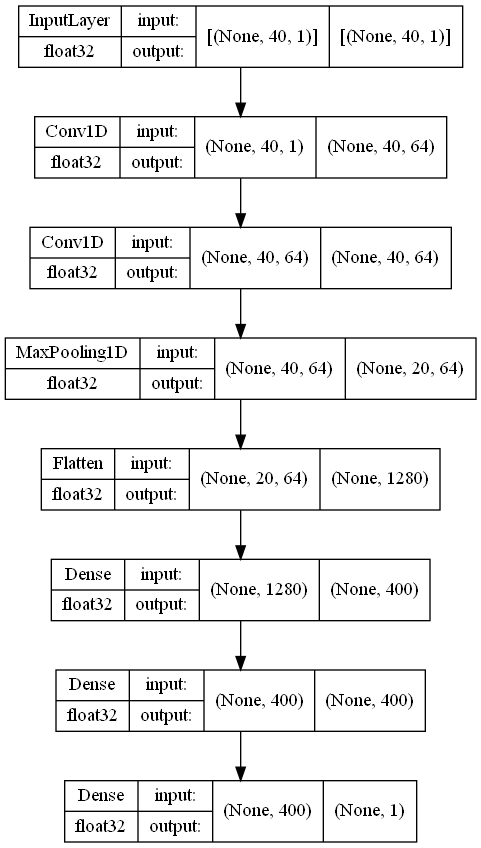
\includegraphics[scale=0.50]{img/esquemaPequenoM1.png}
		\caption{Visual representation of the first model.}
	\end{figure}
	
	Right after implementing the model there are several hyper parameters that need to be tuned so that the model can be compiled and trained, this are often selected by trial and error as well as the previous experience of the person in charge of the implementation of the NN. It was at this point in time, when I was going to start trying several configurations for the hyper parameters that the fist problem arose, \hyperref[sec:explodingGradientProblem]{\textbf{The Exploding Gradient Problem}}.
	
	After solving the issues with the gradient I was finally able to train the network and start establishing the hyperparameters, nonetheless after several trials I started to realize that no there was another issue, this time the algorithm was suffering of overfitting, due to the a problem with the balance of the Data. This issue is further addressed in the subsection of \hyperref[sec:problemUnbalanceData]{\textbf{The Problem With the Balance of the Data}}.
	
	As for the hyper parameters selected for the model I will now explain which ones did I choose when considering the first model or binary classification model as it only had two classes, later on I will explain any changes that came through with the second model or the multi class classification model. As for the binary model I chose the following:
	
	The Loss: the loss of a training process is a hyperparameter that serves both as information for the developer on the evolution of the training process and also as a keystone of the training process by indicating the algorithm how of its presictions are from the actual values on the training and validation sets, each one of those having their own value. As for what to use in the loss function there are many possible metrics, that keras classifies in three main groups:\cite{kerasDocs}
	
	\begin{itemize}
		\item \textbf{Probabilistic}: which focus on implementing formulas that extract the loss value from the probabilities of the different possible events. For example this would be the formula corresponding to one of the many probabilistic losses known as the binary crossentropy.\cite{binnaryCrossentropy}
		
		\[ H_p(q) = -(1/n) \sum y_i * log(p(y_i)) + (1-y_i)*log(1-p(y_i)) \]
		
		\item\textbf{Regression}: which focus on utilizing the estimators, mainly the mean error, to provide the loss value for the given predictions. For example the next equation corresponds to the mean square error loss function, which belongs to this group:
		
		\[ MSE = 1/n \sum(y - \hat y))^2 \]
		
		Where y is the actual value and $\hat y$ its predicted counterpart.
		
		
		\clearpage
		
		\item\textbf{Hinge}: which focus on the implementation of a margin or distance from the classification boundary to establish the loss values for the given predictions, this methods are most utilized for "maximum-margin" classification mainly in Support Vector Machines (SVMs). One example of a hinge loss formula would be:
		
		\[ l(y) = max(0,1 - t * y)\]
		
	\end{itemize}

	According to the previous explanation for the loss I tried with both the binary and categorical crossentopries, but the categorical did not seem to be adequate for this problem mainly due to the fact that in the bigger models in tended to 0 way too fast. Anyway that makes sense as in a binary classification problem such as ours it is most often recommended to utilize the binary cross entropy while the categorical one is left for use in multi class classification problems.
	
	The optimizer: there are several optimizers provided by the keras api that we could implement in our project, nonetheless the two most comonly used ones are the RMSprop and the Adam optimizers.
	
	There is a problem that all optimizers need to face, that been the fact that gradients may vary big magnitudes during the training if the network. This implies that for really small gradients the algorithm learning rate becomes awfully slow and for the biggest ones it could lead to an impossibility of learning for the algorithm due to it taking steps to big to archive the optimal solution.
	
	\begin{figure}[H]
		\centering
		\label{learningRates}
		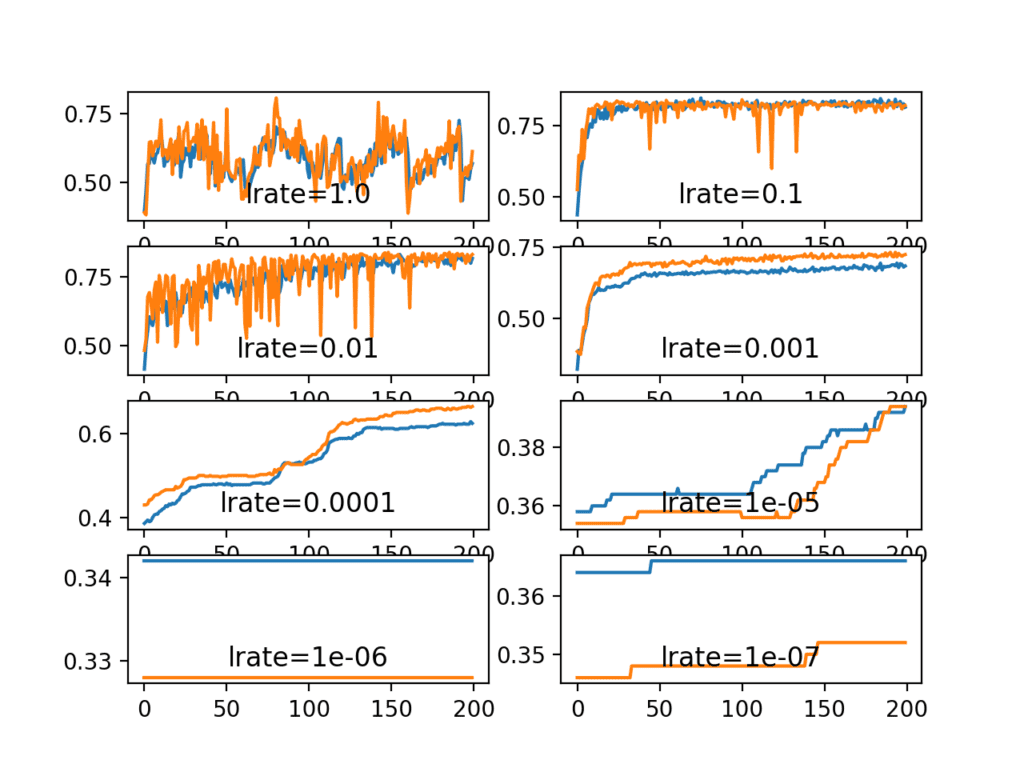
\includegraphics[scale=0.3]{img/learningRates.png}
		\caption{Effects of different learning rates on the learning process of a model. \cite{learningRates}}
	\end{figure}
	
	
	\begin{itemize}
		\clearpage
		\item \textbf{RMSprop}: focuses on dampening the oscillations of the loss function by adjusting the learning rate for the different parameters individually and dynamically according to the root mean square of the component of the gradient relative to the parameter that is been adjusted. This optimizer implements the following formulas for each parameter named $w^j$, where the super index j has been eliminated to help with readability: \cite{RMSprop}
		
		
		\[v_t = pv_{t - 1} + (1-p)*(g_t)^2\]
		
		\[ \Delta w_t = - (n/\sqrt{v_t + \epsilon})*g_t\]
		
		\[ w_{t+1} = w_t + \Delta w_t\]
		With:
		
		n: Initial learning Rate
		
		$v_t$: Exponential Average of squares of gradients
		
		$g_t$: Gradient at time t along $w^j$ 
		
		p, $\epsilon$: Hyperparameters generally chosen to be 0.9 and 1e-10 respectively.
		
			\vspace{5mm}
			
		\item \textbf{Adam}: this heuristic combines properties of the previously described RMSprop and the Momentum approach to learning optimization, which focuses on accelerating the search in the direction of the minima rather than on preventing the oscillations like RMSprop. This method implements the following equations for each parameter named $w^j$, where the super index j has been eliminated to help with readability:
		
		\[v_t = \beta_1 * v_{t-1} - (1- \beta_1) * g_t \]
		
		\[s_t = \beta_2 * s_{t-1} - (1- \beta_2) * (g_t)^2 \]
		
		\[ \Delta w_t = - n( v_t/\sqrt{s_t + \epsilon})*g_t\]
		
		\[ w_{t+1} = w_t + \Delta w_t\]
		
		With:
		
		n: Initial learning Rate
		
		$g_t$: Gradient at time t along $w^j$
		
		$v_t$: Exponential Average of gradients along $w^j$
		
		$s_t$: Exponential Average of squares of gradients along $w^j$
		
		$\beta_1,\beta_2, \epsilon$: Hyperparameters generally chosen to be 0.9, 0.99 and 1e-10 respectively.
		
	\end{itemize}

	After making several trials with both models I did not see a great impact in using any of them for the optimizer of the model and so I chose Adam as it is becoming more popular as of late and it theatrically possesses the qualities of RMSprop and adds to them the benefits of momentum.
	 	
	 When facing the problem of the overfitting of the model that i attributed to the quality and quantity of the data ans is further developed in the \hyperref[sec:problemUnbalanceData]{\textbf{The Problem With the Balance of the Data}} section, I also tried adding regularization to the model as a way of fighting against the overfitting.
	 
	 Regularization techniques work by fitting the function of the given layer to the training set. In my case I tried applying regularization to the kernel, bias and activity of the dense layers of the model of both types, L1 and L2, but it did not have any significant impact on the outcomes of the training process of the model. The two models implement the following equations:\cite{regularization}
	 
	 
	 \[L1 = \sum{(Y_i - \sum{X_{ij}\beta_j})^2 + \lambda \sum{|\beta_j|}} \]
	 
	 \[L2 = \sum{(Y_i - \sum{X_{ij}\beta_j})^2 + \lambda \sum{{\beta_j}^2}} \]
	 
	
	\clearpage
	
	\subsection{The Exploding Gradient Problem.}
	\label{explodingGradientProblem}
	
	This problem and its counterpart the Vanishing gradient problem happens due to the shape of some of the activation functions often implemented, such as the Sigmoid function. 
	
	\vspace{5mm}
	
	\begin{figure}[H]
		\label{SigmoidAndDerivative}
		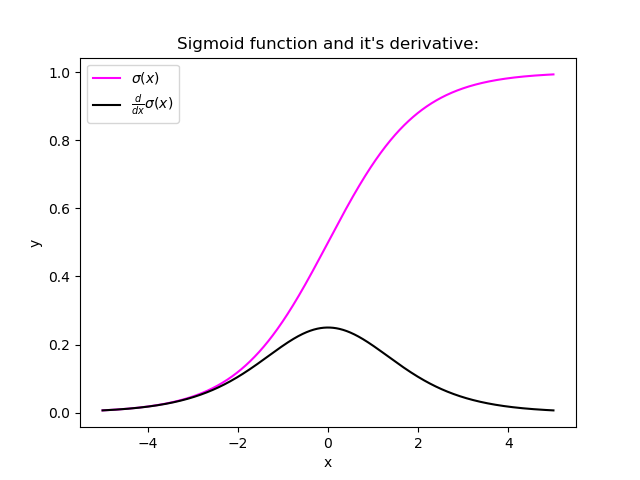
\includegraphics{img/plots/Sigmoid.png}
		\caption{Sigmoid function and it´s derivative. \cite{Vanishing}}
	\end{figure}

	\vspace{5mm}
	
	As it can be appreciated in the chart this function saturates when fed with larger inputs (both negative and positive). This causes that, in some scenarios such as ours, as the back propagation function propagates through the different layers the gradient gets bigger each time to the point where it causes very large updates of the weights and thus makes the gradient descent diverge. This when applied to computing can be detected by some weights becoming incredibly high numbers or even NaN which on time causes an exception as we can see in the logs presented. The other problem that could occur is the aforementioned Vanishing gradient problem, but this is often related to an stall in the training of the NN by the weights becoming too small and so due to the percepted effects of the problematic it seems more plausible for it to be caused by Exploding Gradient instead.
	
	Other posible explanations for the apparition of this problem are the initial weights causing a big loss and the network been way too big for the problem at hand, in any case there are several methods to prevent the negative effects this problem carries to the model and those are:\cite{Vanishing}
	
	
	\begin{itemize}
		
		\item Setting the kernel\_initializer, the function implemented for the initial weight generation, to use the Glorot inicialization, named after its author, which works with the variance of the gradients that come in and out of a layer as well as the variances of every layer´s inputs and outputs to try to make them as close to each other as possible.
		
		\item To normalize the output of each layer before imputing it to the next one, by adding several BatchNormalization keras´s layers between the different layers of the model.
		afortunadamente
		\item To clip the gradients during the backpropagation algorithm so that it can not exceed a threshols that is stablishes as a hyperparameter by adding the clipnorm parameter to the optimizer.
		
	\end{itemize}

	I tried implementing the previously mentioned techniques but only the clipping of the gradient had the desired effects by preventing it from Exploding. Nonetheless I suspect that clipping the gradient might have negative effects later on in the process and 
	fortunately In my trial and error process for solving the Exploding Gradient process I also realized that this problem can be solved by diminishing the size of the neuronal network. Taking in count my suspicions I decided to carry the application process with both, the clipped version of the original NN and the smaller version which has the following code:
	
		
	\vspace{5mm}
	
	\begin{lstlisting}[language=Python]
		
		model = Sequential() 
		model.add(Conv1D(input_shape=TRAIN_ARRAY.shape[1:],filters=64,kernel_size=(3),padding="same", activation="relu"))
		model.add(Conv1D(filters=64,kernel_size=(3),padding="same", activation="relu"))
		model.add(MaxPool1D(pool_size=(2),strides=(2),padding="same"))
		model.add(Flatten())
		model.add(Dense(units=400,activation="relu", kernel_regularizer='l2'))
		model.add(Dense(units=400,activation="relu", kernel_regularizer='l2'))
		model.add(Dense( units=1, activation= "softmax"))
	\end{lstlisting}
	
	\vspace{5mm}
	
	It is also relevant to say that at this point in time both archived the same results as both were equally affected by the next problem that will be addressed, but I keep them to analyze any changes in their performance that could lead to a model surpassing the other after the several problems are solved.
	
	In the following section, The Problem With the Balance of the Data, I will continue with the overffiting problem that arose due to the unbalance of the data.
	
	\clearpage
	
	\subsection{The Problem With the Balance of the Data}
	\label{problemUnbalanceData}
	
	Most often machine learning algorithms do not handle biased data very well, as most expect a normal distribution of the samples utilized on the training process. Nonetheless there are cases where using balanced data for the training is found to be impossible, in those instances we can have several problems with the model.
	
	When the model performs well on the training data, but it does not generalize well, it is said to be overfitting, in our case although the performance of both models seems to be relatively good when generalizing, with both the accuracy and binary accuracy of the two model going from 0.8193 on the training set to 0.9189 on the validation one, when checking the confusion matrix for the model we can clearly see the issue. Overfitting happens when the model is too complex relative to the amount and noisiness of the training data and given the disparity on the numbers of the members of the different classes that we posses within our dataset it makes perfect sense for the model to arrive to the conclusion that assuming all to be positive yields rather impressive results specially when implementing the binary cross-entropy as the function of loss for the training of the data.
		
		\vspace{15mm}
	
	\begin{lstlisting}[language=Python]
		
		from sklearn.metrics import ConfusionMatrixDisplay
		
		pred = model.predict(TEST_ARRAY)
		ConfusionMatrixDisplay.from_predictions(pred, TEST_LABELS_ARRAY)
		plt.show()
	\end{lstlisting}

	\vspace{5mm}

	\begin{figure}[H]
		\centering
		\label{UnbalancedConfusionMatrix}
		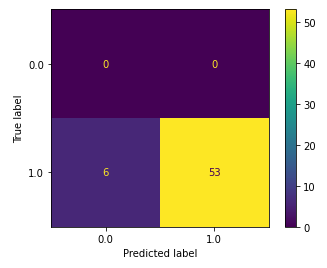
\includegraphics[scale=1.2]{img/plots/matrizDeConfusion.png}
		\caption{Confusion Matrix for the predictions of the model trained with unbalanced data.}
	\end{figure}
	\vspace{5mm}

	As we can see on Figure 9, the model comes to the realization that it is best to always classify the person as positive, this is caused by the unbalances nature of the data where for the training set, and it is the same for validation and test, the number of positives is 195 where as the number of negatives is 43 meaning that around 82\% of the instances within the set are labeled as positive in Parkinson´s Disease.
	
	\begin{figure}[H]
		\centering
		\label{UnbalancedTrainDataSet}
		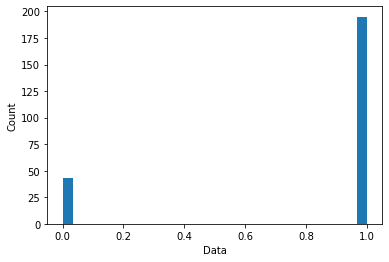
\includegraphics{img/plots/unbalancedTrainDataGraph.png}
		\caption{Label distribution for the unbalanced train data set.}
	\end{figure}
	
	This on time causes a situation of overfitting for which I found two possible solutions.
	
	\begin{itemize}
		
		\item Implementing Weighted classes with SkLearn
		
		\item Stablishing A clasification System Based on the UPDRS
		
	\end{itemize}
	
	\clearpage
	
	\subsubsection{Implementing Weighted classes with SkLearn}
	
	
	Class weights are values given to the different classes that constitute the outcome of the classification algorithm according to their representation within the training set of data. Usually the minority classes will be assigned bigger weights while the majority ones will often have a weight smaller than one. This weights are later fed to the training algorithm and are used to penalize the misclassification of the elements of the minority classes while also lessening the importance of this same misclassification for the elements that belong to the majority classes. In this way we can make the algorithm adapt to the skewness proper to the biased distribution.
	
	To be more precise when implementing "balanced" class weights, the weights values assigned to each class are inversely proportional to the frequency of that given class in the data set.\cite{classWeights}
	
	\[ wj = n\_samples / (n\_classes * n\_samplesj) \] 
	
	According to the previous explanation the idea is to give different weights to the different classes coming out of the classification algorithm, to calculate the corresponding weights, which are based on the training data, there is a function in the utils package from sklearn that will do the job:
	
	\vspace{5mm}
	
	\begin{lstlisting}[language=Python]
			
		from sklearn.utils.class_weight import compute_class_weight
		import numpy as np
		
		res = compute_class_weight(class_weight = 'balanced', classes = np.unique(TRAIN_LABELS), y = TRAIN_LABELS);
		balanced_dict = dict(zip(np.unique(TRAIN_LABELS), res))
		print(balanced_dict)
		
		>> {0: 2.7674418604651163, 1: 0.6102564102564103}
	
	\end{lstlisting}

	\vspace{5mm}
	
	As for the application of the classes to the model it is as simple as feeding the balanced\_dict as input value for the  class\_weight parameter within the fit function of the model.
	
	Unfortunately this method did not seem to have any mayor effects on any of the models utilizes for this implementation. Al thou according to the the loss of the model, which I established to be de binary\_crossentropy, both models do try to perform better during their training process, both get stuck from the very beginning in the idea that saying that every patient is sick with Parkinson´s disease is the best outcome. It is relevant to acknowledge that while in some problems the accuracy alone could be a good enough metric to stablish the correctness of the algorithm, thus markin ours who has an accuaricy above 80\% as a good system, in our scenario the acuracy alone falls short and the confusion matrix seems to be far more representatice. With this in mind it would seem that this classification approach is a failure and thus I propose a new approach in the following section.
	
	As for the reasons behind the failure of out first model those seem yet unclear, although there are several conclusions that could be extracted from the previous process.
	
	The first one is that the failure of this model does not depend on its size as two model of similar structure yet very different size where compared. With the objective of finding out if the failure of the fist model was due to its size I even tried with smaller models composed of only dense layers but there where no perceptible signs of change further than an increase in the loss when training the models, which seemed to indicate that the models where getting too small to be able to learn given the dimensionality of the problem.
	
	The second option I see would be that the problem is within the data utilized for the training of the dataset, seen how I extensively treated the data to try and make it as clean as possible for its use in the training process of the models I am more inclined to say that the impossibility of this model to learn given the data that we posses was due to the noisiness of the data or its number of samples, that got heavily reduced during the data cleanse and normalization processes. It could have therefore been a good idea to try and reduce the amount of data eliminated in this process or try and recollect or generate new stances that could enlarge the different data sets that take part on the training and evaluation of the model.
	
	\clearpage
	
	\subsubsection{Stablishing A clasification System Based on the UPDRS}
	
	The UPDRS or Unifies Parkinson´s Disease Rating Scale has several measurements that help health experts asses the patient´s mental state, their conduct and mood, as well as the state of their motor functions and their ability to realize every day tasks. This scale if often used to asses the effects of the medication on a patient or establish the degree of development of the disease they are subjected to and the effect it has on their live.
	
	In our initial dataset there are several attributes that relate to the UPDRS scale which on time will allow as to establish different groups according to the level of deterioration the sickness has caused the patient, which hopefully will allow as to have better balanced groups over which to train a model.
	
	\vspace{5mm}
	
	\begin{tabularx}{1\textwidth} { 
		| >{\raggedright\arraybackslash}X 
		| >{\raggedright\arraybackslash}X 
		| >{\raggedright\arraybackslash}X 
		| >{\raggedright\arraybackslash}X |}
	\hline
	\textbf{Name} & \textbf{Description} & \textbf{Type} & \textbf{Units} \\
	\hline
	memory  & PDRS Q1 & integer & 0-4 \\
	\hline
	hallucinations  & PDRS Q2 & integer & 0-4 \\
	\hline
	mood  & PDRS Q3 & integer & 0-4 \\
	\hline
	motivation  & PDRS Q4 & integer & 0-4 \\
	\hline
	speech  & PDRS Q5 & integer & 0-4 \\
	\hline
	saliva  & PDRS Q6 & integer & 0-4 \\
	\hline
	swallowing  & PDRS Q7 & integer & 0-4 \\
	\hline
	handwriting  & PDRS Q8 & integer & 0-4 \\
	\hline
	cutting\_food  & PDRS Q9 & integer & 0-4 \\
	\hline
	dressing  & PDRS Q10 & integer & 0-4 \\
	\hline
	hygiene  & PDRS Q11 & integer & 0-4 \\
	\hline
	turning\_in\_bed  & PDRS Q12 & integer & 0-4 \\
	\hline
	falling  & PDRS Q13 & integer & 0-4 \\
	\hline
	freezing  & PDRS Q14 & integer & 0-4 \\
	\hline
	walking  & PDRS Q15 & integer & 0-4 \\
	\hline
	tremors  & PDRS Q16 & integer & 0-4 \\
	\hline
	numbness  & PDRS Q17 & integer & 0-4 \\
	\hline
\end{tabularx}
	
	\clearpage
	
	Although not all the attributes related to the UPDRS scale can be easily related to the audio data the main idea is that the scale gives a rough level of deterioration for the patient, and it can be argued that this deterioration caused bu the sickness is bound to affect the vocal qualities of the patient. This is none the less a hypotesis of mine which is yet to be tested and therefore the model could fail due to this factors not been significantly related.
	
	The first step before starting to generate the model would be to create the new function to generate the labels and evaluating the distribution of the data over the new classes to see if this approach seems relevant.
	
	As for the criteria of the classes I will be adding the scores for the patient in all the attributes relates to the UPDRS and adapt the boundaries of the classes as needed to help the even distribution of the instances of the data.
	
	\vspace{10mm}
	
	\begin{figure}[H]
		\centering
		\label{UPDRSSumDistribution}
		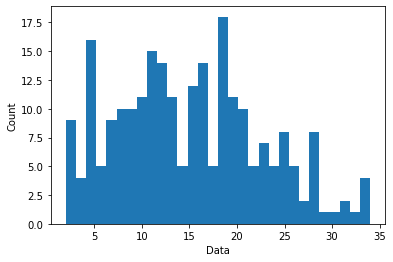
\includegraphics{img/plots/UPDRSsum.png}
		\caption{Distribution for the sum of the different attributes associated to the UPDRS within the data set.}
	\end{figure}
	
	Based on the distribution of the variable just shown in the graph above I adjusted the previous getDataFrameLabels function in order to produce classes with more or less the same number of samples. I also decided to make a group composed of all the individuals who have not been diagnosed with the disease but due to its size I will try both, training the model with this class and removing it, for I think it could have a negative effect in the model.
	
	\clearpage
	
	\begin{lstlisting}[language=Python]
		
		def getDataFrameLabels(data_frame):
			C0 = [1,0,0,0]
			C1 = [0,1,0,0]
			C2 = [0,0,1,0]
			C3 = [0,0,0,1]
			data_labels = []
			data_frame.head()
			heads = ["memory", "hallucinations", "mood", "motivation", "speech", "saliva", "swallowing", "handwriting","dressing", "cutting_food", "hygiene", "turning_in_bed", "falling", "freezing", "walking", "tremors", "numbness" ]
			for index, row in data_frame.iterrows():
			addition = 0
			for elem in heads:
				addition = addition + row[elem]
				if (addition == 0):
					data_labels.append(C0)
				elif (addition > 0 and addition <= 10):
					data_labels.append(C1)
				elif (addition > 10 and addition <= 17):
					data_labels.append(C2)
				else:
					data_labels.append(C3)
			return data_labels
	\end{lstlisting}
	
	
	\begin{figure}[H]
		\centering
		\label{UPDRSSumDistributionClasses}
		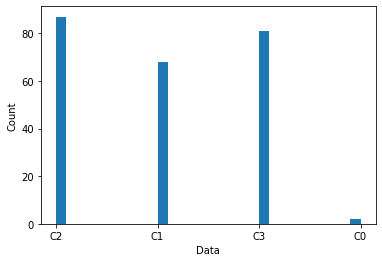
\includegraphics[scale=0.95]{img/plots/UPDRSsumClasses.png}
		\caption{Distribution for the classes created based of sum of the different attributes associated to the UPDRS within the data set.}
	\end{figure}

	\vspace{10mm}
	
	With this new classes we will have a more uniform set of classification options for the model which should make it so that we surpass the problem of the imbalance of the data that stopped our first model. Speaking in percentages the C1 contains 33.19\% of the total samples, C2 contains 33.61\% and C3 contains 32.35\% while C0 contains less than a 1\% of the samples thus been unreasonably unbalanced. I will try to keep it as ideally it would be very interesting for the model to be able to classify non ill people as well as the level of deterioration caused in Parkinson´s patients, but due to the small number of samples we have for this group I doubt this will be possible.
	
	First I tried to train a model based on the VGG-16 architecture, with the same structure as the bigger of the two models presented in the previous binary classification approach but changing the number of neurons in the output layer so that it would adapt to the new structure I was aiming for:
	
		\vspace{10mm}
	
	\begin{lstlisting}[language=Python]
		
		model = Sequential()
		model.add(Conv1D(input_shape=TRAIN_ARRAY.shape[1:],filters=64,kernel_size=(3),padding="same", activation="relu"))
		model.add(Conv1D(filters=64,kernel_size=(3),padding="same", activation="relu"))
		model.add(MaxPool1D(pool_size=(2),strides=(2)))
		model.add(Conv1D(filters=128, kernel_size=(3), padding="same", activation="relu"))
		model.add(Conv1D(filters=128, kernel_size=(3), padding="same", activation="relu"))
		model.add(MaxPool1D(pool_size=(2),strides=(2)))
		model.add(Conv1D(filters=256, kernel_size=(3), padding="same", activation="relu"))
		model.add(Conv1D(filters=256, kernel_size=(3), padding="same", activation="relu"))
		model.add(Conv1D(filters=256, kernel_size=(3), padding="same", activation="relu"))
		model.add(MaxPool1D(pool_size=(2),strides=(2)))
		model.add(Conv1D(filters=512, kernel_size=(3), padding="same", activation="relu"))
		model.add(Conv1D(filters=512, kernel_size=(3), padding="same", activation="relu"))
		model.add(Conv1D(filters=512, kernel_size=(3), padding="same", activation="relu"))
		model.add(MaxPool1D(pool_size=(2),strides=(2)))
		model.add(Conv1D(filters=512, kernel_size=(3), padding="same", activation="relu"))
		model.add(Conv1D(filters=512, kernel_size=(3), padding="same", activation="relu"))
		model.add(Conv1D(filters=512, kernel_size=(3), padding="same", activation="relu"))
		model.add(MaxPool1D(pool_size=(2),strides=(2)))
		model.add(Flatten())
		model.add(Dense(units=4096,activation="relu"))
		model.add(Dense(units=4096,activation="relu"))
		model.add(Dense(units=4, activation="softmax"))
	\end{lstlisting}

		\vspace{10mm}

	While the model was mostly identical I had to change my selection of the loss function and the metrics, so I decided to utilize the aforementioned categorical\_crossentropy  (in section 4 Implementation of the CNN) as my loss function and for the metrics I implemented the Accuracy and Categorical Accuracy as well as the multiclass confusion matrix that I was able to generate by implementing the confusion\_matrix function from the metrics module in the sklearn library:
	
		\clearpage
	
	\begin{lstlisting}[language=Python]
		
		from sklearn import metrics
		preds = model.predict(TEST_ARRAY)
		matrix = metrics.confusion_matrix(TEST_LABELS_ARRAY.argmax(axis=1),
		preds.argmax(axis=1))
		matrix
		
		>> array([[12,  0,  7],
				  [ 5,  0, 12],
				  [ 8,  0, 15]], dtype=int64)
				  
	 \end{lstlisting}
 
		\vspace{10mm}	
		
	The previous example of the implementation of the confusion\_matrix function was done over the test data set and having merged the C0 class with the C1.
	
	The problem with this first model was that it overfitted the training set, while I could have tried to solve that with any of the means presented in section 4.2 I first decided to try with and adaptation of the smaller model implemented in the previous binary classification approach and after some fine tuning this new model yielded better results.
	
		\clearpage
	
	\begin{lstlisting}[language=Python]
		
		model = Sequential() 
		model.add(Dropout(.2, input_shape=TRAIN_ARRAY.shape[1:]))
		model.add(Conv1D(filters=64,kernel_size=(3),padding="same", activation="relu"))
		model.add(Conv1D(filters=64,kernel_size=(3),padding="same", activation="relu"))
		model.add(MaxPool1D(pool_size=(2),strides=(2),padding="same"))
		model.add(Conv1D(filters=128, kernel_size=(3), padding="same", activation="relu"))
		model.add(Conv1D(filters=128, kernel_size=(3), padding="same", activation="relu"))
		model.add(MaxPool1D(pool_size=(2),strides=(2)))
		model.add(Flatten())
		model.add(Dense(units=700,activation="relu"))
		model.add(Dense(units=700,activation="relu"))
		model.add(Dense( units=4, activation= "softmax"))
		
	\end{lstlisting}
	
	\vspace{10mm}
	
	At the beginning the model was of the same size that the one presented as the second model in the binary classification section. This first attempt on the model stagnated on around a 30\% crossentropy Accuracy for all train validation and test, in order to solve this stagnation of the learning process I tried changing several hyperparameters and ended up with the model you see above but without any regularization or dropout.
	
	This is an example of overfitting caused by the previous model with no regularization or dropout.
	
		\vspace{5mm}
	\begin{lstlisting}[language=Python]
		
		model.evaluate(TRAIN_ARRAY, TRAIN_LABELS_ARRAY)
		
		>> 8/8 [==============================] - 0s 6ms/step - loss: 3.5593e-05 - categorical_accuracy: 1.0000 - accuracy: 0.0914
	\end{lstlisting}

	\clearpage
	
	\begin{lstlisting}[language=Python]
		
		model.evaluate(VALIDATION_ARRAY, VALIDATION_LABELS_ARRAY)
		
		>> 3/3 [==============================] - 0s 5ms/step - loss: 9.1578 - categorical_accuracy: 0.4189 - accuracy: 0.0405
	\end{lstlisting}
	
	\begin{lstlisting}[language=Python]
		
		model.evaluate(TEST_ARRAY, TEST_LABELS_ARRAY)
		
		>> 2/2 [==============================] - 0s 6ms/step - loss: 37.8091 - categorical_accuracy: 0.3051 - accuracy: 0.0381
	\end{lstlisting}
		\vspace{5mm}
	
	As this newer and bigger model ended up overfitting the training dataset I proceeded to try implementing both a Dropout layer and L2 regularization in the Dense layers, in the end what yielded better results was leaving the Dropout layer without any kind of regularization.
	
	At this point I decided to implement the ModelCheckpoint class from keras library that allows as to save and load the "best" epoch of the training process instead of the last one. In our case the epoch considered to be the best would be the one with the lowest loss on its validation set as choosing the one with the highest validation crossentropy accuracy seemed to yield good results for train and test but significantly worse in the test dataset.
	
	This is an example of the performance of the model with the dropout layer included and the validation crossentropy accuracy as indicator of the quality of the epoch.
	
		\vspace{5mm}
	\begin{lstlisting}[language=Python]
		
		model.evaluate(TRAIN_ARRAY, TRAIN_LABELS_ARRAY)
		
		>> 8/8 [==============================] - 0s 6ms/step - loss: 0.9080 - categorical_accuracy: 0.5252 - accuracy: 0.0000e+00
	\end{lstlisting}
	
	\clearpage
	
	\begin{lstlisting}[language=Python]
		
		model.evaluate(VALIDATION_ARRAY, VALIDATION_LABELS_ARRAY)
		
		>> 3/3 [==============================] - 0s 5ms/step - loss: 1.1463 - categorical_accuracy: 0.5541 - accuracy: 0.0000e+00
	\end{lstlisting}
	
	\vspace{5mm}
	
	\begin{lstlisting}[language=Python]
		
		model.evaluate(TEST_ARRAY, TEST_LABELS_ARRAY)
		
		>> 2/2 [==============================] - 0s 7ms/step - loss: 2.1517 - categorical_accuracy: 0.3390 - accuracy: 0.0085
	\end{lstlisting}
	\vspace{5mm}
	
	This is an example of the performance of the model with the dropout layer included and the validation loss as indicator of the quality of the epoch.
	
	\vspace{5mm}
	\begin{lstlisting}[language=Python]
		
		model.evaluate(TRAIN_ARRAY, TRAIN_LABELS_ARRAY)
		
		>> 8/8 [==============================] - 0s 6ms/step - loss: 1.0641 - categorical_accuracy: 0.3992 - accuracy: 0.0000e+00
	\end{lstlisting}
	
	\vspace{5mm}
	
	\begin{lstlisting}[language=Python]
		
		model.evaluate(VALIDATION_ARRAY, VALIDATION_LABELS_ARRAY)
		
		>> 3/3 [==============================] - 0s 5ms/step - loss: 1.0902 - categorical_accuracy: 0.3378 - accuracy: 0.0000e+00
	\end{lstlisting}

	\vspace{5mm}
	
	\begin{lstlisting}[language=Python]
		
		model.evaluate(TEST_ARRAY, TEST_LABELS_ARRAY)
		
		>> 2/2 [==============================] - 0s 6ms/step - loss: 1.9819 - categorical_accuracy: 0.3390 - accuracy: 0.0085
	\end{lstlisting}
	
	\vspace{5mm}
	
	Ir order to evaluate the impact of several of the techniques applied to the data as well as the fact that many instances where eliminated during the data cleaning process I decided to do some final trials:
	
	First I decided to not normalize the data to see haw the normalization affects the learning process of the network.
	
	\vspace{5mm}
	\begin{lstlisting}[language=Python]
		
		model.evaluate(TRAIN_ARRAY, TRAIN_LABELS_ARRAY)
		
		>> 8/8 [==============================] - 0s 6ms/step - loss: 1.0161 - categorical_accuracy: 0.4790 - accuracy: 0.0000e+00
	\end{lstlisting}
	
	\vspace{7mm}
	
	\begin{lstlisting}[language=Python]
		
		model.evaluate(VALIDATION_ARRAY, VALIDATION_LABELS_ARRAY)
		
		>> 3/3 [==============================] - 0s 5ms/step - loss: 1.0381 - categorical_accuracy: 0.4459 - accuracy: 0.0034
	\end{lstlisting}
	
	\vspace{7mm}
	
	\begin{lstlisting}[language=Python]
		
		model.evaluate(TEST_ARRAY, TEST_LABELS_ARRAY)
		
		>> 2/2 [==============================] - 0s 7ms/step - loss: 1.1821 - categorical_accuracy: 0.3390 - accuracy: 0.0000e+00
	\end{lstlisting}
	
	\vspace{5mm}
	
	And finally I decided to give default values to the NaN and Null cells of the dataset to see the impact that the decrement in the number of instances for the data sets might have caused. We must not forget that by giving default values to this attributes I am also adding noise to the dataset and that could end up causing travel as well. For this experiment I normalized the data although I did try with all the data and without normalization, it did not make a difference.
	
	\clearpage
	\begin{lstlisting}[language=Python]
		
		model.evaluate(TRAIN_ARRAY, TRAIN_LABELS_ARRAY)
		
		>> 15/15 [==============================] - 0s 6ms/step - loss: 0.8312 - categorical_accuracy: 0.6717 - accuracy: 0.0000e+00
	\end{lstlisting}
	
	\vspace{7mm}
	
	\begin{lstlisting}[language=Python]
		
		model.evaluate(VALIDATION_ARRAY, VALIDATION_LABELS_ARRAY)
		
		>> 5/5 [==============================] - 0s 6ms/step - loss: 0.8420 - categorical_accuracy: 0.6783 - accuracy: 0.0000e+00
	\end{lstlisting}
	
	\vspace{7mm}
	
	\begin{lstlisting}[language=Python]
		
		model.evaluate(TEST_ARRAY, TEST_LABELS_ARRAY)
		
		>> 4/4 [==============================] - 0s 6ms/step - loss: 0.8810 - categorical_accuracy: 0.6579 - accuracy: 0.0000e+00
	\end{lstlisting}
	
	\vspace{5mm}
	
	\clearpage
	
	\section{Conclusions}
	
	While I had my reasons for doing so, given the limited data at my disposal I would say that my data cleaning process was too harsh. The problem with allowing data of doubtful quality to stay in the dataset is that it could create noise or even make the Neural Network find patterns that are false, given that the data is actually wrong, and therefore it is risky. This could on time have a massive negative impact in the training process and future predictions of the model.
	
	I would say that the implementation of the binary classification model failed mainly due to the lack of samples without the disease, problem that might have been related to the cleaning process. If I were to leave all instances the difference between classes would have been of 5.546 to 1 people having Parkinson´s Disease in the entirety of the data, which while already unbalanced had significantly more samples of the healthy group.
	
	This claim is further supported by the lack of results yielded by the different methodologies applied to try and solve the issue and the fact that even for the second model the best results obtained are those from the trial without dropping any undefined values.
	
	As per the second take with the multiclass classification model the more uniform distribution of samples over the different output classes allowed for a model that could yield some results. Nonetheless those results ended up not been too promising.
	
	\vspace{10mm}
	
	\begin{table}[h]
		\centering
		\resizebox{\textwidth}{!}{%
			\begin{tabular}{cccc}
				\hline
				Case & Train Categorical Accuracy & Validation Categorical Accuracy & Test Categorical Accuracy \\ \hline
				\begin{tabular}[c]{@{}c@{}}Second multiclass model\\  with no regularization\end{tabular} & 1.0000 & 0.4189 & 0.3051 \\ \hline
				\begin{tabular}[c]{@{}c@{}}Second multiclass model with \\ Dropout and checkpoint based on \\ Categorical Accuracy\end{tabular} & 0.5252 & 0.5541 & 0.3390 \\ \hline
				\begin{tabular}[c]{@{}c@{}}Second multiclass model with\\  Dropout and checkppoint \\ based on Loss function\end{tabular} & 0.3992 & 0.3378 & 0.3390 \\ \hline
				\begin{tabular}[c]{@{}c@{}}Second model with \\ unormalized data\end{tabular} & 0.4790 & 0.4459 & 0.3390 \\ \hline
				\begin{tabular}[c]{@{}c@{}}Second model with \\ undetermined values\end{tabular} & 0.6717 & 0.6783 & 0.6579 \\ \hline
			\end{tabular}%
		}
		\caption{Table with all the results for the trials that have been done over the second model of the multiclass clasification approach.}
		\label{MulticlassSecondModelResultTable}
	\end{table}
	
	\vspace{10mm}
	
	In the end I merged C0 (the class that contained all instances with 0 on every aspect of the UPDRS and therefore healthy) with C1 (the class containing the instances of the data with the lowest range for the sum of the values of the different UPDRS related attributes), due to the low representation of the C0 class, that would make it really hard or even impossible for the network to establish patterns, and the fact that there were no instances of C0 on the test dataset.
	
	Seen how all the different trials yielded very similar results for their Test metrics except for the final one, that included the rows with one or more undefined values on them, which actually doubled the other trials test categorical accuracy, I would say that the main reason for the model to get stagnated soon on the learning process was the lack of data that made it impossible for the model to learn the patters within. As we can see this lack of data not only improves the generalization capabilities of the model but añso its learning abilities as the validation and train metrics where the highest and second highest from all trials respectively (including the overfitting ones).
	
	
	
	\clearpage
	
	\subsection{Possible Future Work Lines}
	
	One of the main problems faces in this paper was the availability of trust worthy data, this on time could lead to two possible lines of work that would significantly improve future Machine Learning implementations over smaller datasets such as the one utilized in this paper.
	
	\begin{itemize}
		\item Anomaly detection would allow for a better filter of the data, helping identify any instances that need to be removed due to their nature. one of the approaches could be based on unsupervised learning and it works by showing the system mostly normal instances during training, so it learns to recognize them. Later when it comes across a new instance, it should be able to tell whether it is a normal or an anomaly. This could help in cases such as mine where too many instances of the data where taken out during the cleaning process to prevent risks by more accurately marking those that could have a negative effect on the system.
		
		\item Generation of new instances could also be an option and this path has the advantage of allowing projects that start with rather small quantities of data to increase the size of their data frames. In this case I suggest looking into the possibility of implementing GAN (Generative Adversarial Networks) which are becoming more and more popular and could yield interesting results.
		
	\end{itemize}
	
	Finally I can think of one last way of further developing this project and that would be to try and implement different types of Machine Learning Algorithms, in the case of CNN they do take in count the physical proximity of the features within the input to the model and the relation between the attributes that I positioned together might have been too weak, which on time could have hindered the learning of the model. On this bases I think it might be a good idea to investigate the possibility of implementing other ML systems but I will also suggest to focus on Deep Learning as from my knowledge of the problem it seems quite complex.
	
	\clearpage
	
	\subsection{Social Implications}
	
	This End Grade Project is focused on research and therefore iy is hard to argue any direct implications it might have on society. As for the possibility of the outcomes of this project to be implemented in any kind of consumer directed software I would argue that the idea of implementing a system for recognition and diagnosis of Parkinson´s disease through voice recordings that could be generated with a mobile phone could help in the early detection and treatment of Parkinson´s disease, therefore helping people affected by this malady to be recognized sooner and posses an alternative way of assessing the development of the sickness that could ease the number of visits to medics and/or hospitals that this patients require in order to follow up on the development of their sickness. This would ultimately improve their quality of live and help to recognize sooner possible cases as well as easing the development assessment process of the disease.
	
	Unfortunately the outcomes of this paper have not been good enough so that I would suggest implementing any of the models discussed within this pages in any kind of consumer bases application. This paper none the less proves the bases that a categorization Machine Learning based system might be possible using the parametrization of voice recording and some general data (such as age and gender) given that enough data is provided for the training and evaluation of the model.
	
	\clearpage
	
	\section*{Glossary}
	
	\begin{itemize}
		
		\item[] \textbf{CNN:} Convolutional Neural Network
		
		\item[] \textbf{VGG:} Visual Geometry Group CNN architecture
		
		\item[] \textbf{UPDRS:} Unified Parkinson’s Disease Rating Scale
		
		\item[] \textbf{MLS:} Machine Learning Systems
		
		\item[] \textbf{RNN:} Recursive Neuronal Network
		
		\item[] \textbf{ANN:} Artificial Neuronal Network
		
		\item[] \textbf{NN:} Neuronal Network
		
	\end{itemize}
	
	\clearpage
	
	\bibliography{bibliografia.bib}
	
	\bibliographystyle{IEEEtran}
	
\end{document}




